\newpage
\section{The KdV Equation and the Wave Equation}

\subsection{Fundamental solution of the KdV equation}
Last time, we were discussing the $\mathrm{KdV}$ equation
$$
\left(\partial_{t}+\partial_{x}^{3}\right) u=f
$$
We saw that the fundamental solution was given by
$$
\widehat{K}(t, \xi)=e^{i t \xi^{3}}
$$
Taking the inverse Fourier transform in $x$ gives
$$
K(t, x)=\int e^{i\left(t \xi^{3}-x \xi\right)} d \xi
$$
This problem admits a type of scaling. If we want
$$
\left(\partial_{t}+\partial_{x}^{3}\right) u=0
$$
then we can make a change of variables $u(x, t) \mapsto u\left(\lambda x, \lambda^{3} t\right)$. If we want to get rid of the time variable, we can set $\xi=t^{-1 / 3} \xi$, so the integral becomes
$$
\begin{aligned}
K(t, x) &=t^{-1 / 3} \int e^{i \eta^{3}+x / t^{1 / 3} \eta} d \eta \\
&=t^{-1 / 3} K\left(1, x / t^{1 / 3}\right) \\
&=t^{-1 / 3} \operatorname{Ai}\left(x / t^{1 / 3}\right)
\end{aligned}
$$
where
$$
\operatorname{Ai}(x)=\mathcal{F}^{-1}\left(e^{i \xi^{3}}\right)=\int e^{i\left(t\xi^{3}+x \xi\right)} d \xi
$$
In this integral, we have the phase function $\varphi(\xi)=\xi^{3}+x \xi$. The critical points, with $\varphi_{\xi}=0$, are $\xi_{1,2}= \pm \sqrt{-x / 3}$ with $x<0$.

Let's draw a picture of the Airy function; this is real-valued because the equation is real, so the real and imaginary parts of any solution should also be solutions. At $+\infty$, we have no stationary points, so we expect rapid decay. This decay is $O\left(e^{-x^{3 / 2}}\right)$, which one can prove by changing the contour in the integral (to some other integral over a contour in the complex plane).

\begin{figure}[H]
    \centering
    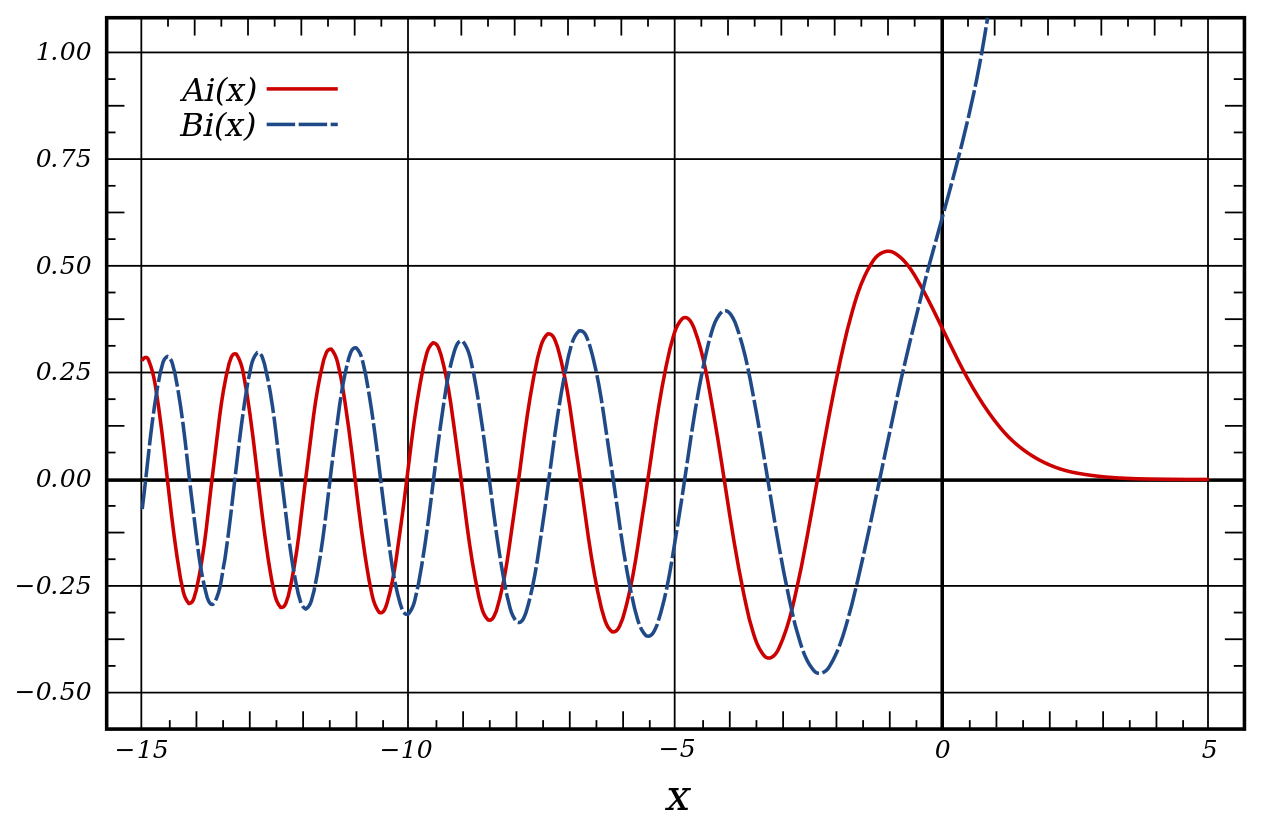
\includegraphics[width=0.8\textwidth]{pics/19-1.png}
\end{figure}

Choose $\xi_1=\sqrt{-x / 3}$, look at the contribution around $\xi_{1}$, and take $2 \mathrm{Re}$.
$$
\varphi(\xi)=\varphi\left(\xi_{1}\right)+\frac{1}{2} \varphi^{\prime \prime}\left(\xi_{1}\right)\left(\xi-\xi_{1}\right)^{2}+\underbrace{O\left(\left(\xi-\xi_{1}\right)^{3}\right)}_{\text {discard }}
$$

We are multiplying two functions, a Gaussian and a function with oscillation.

Recall that $\mathcal{F}^{-1}\left(e^{i \lambda \xi^{2} / 2}\right)=-\frac{1}{(i \lambda)^{n / 2}} e^{i x^{2} /(2 \lambda)} .$ Now obsesrve that the Fouerier transform lets us figure out the integral of a function: $\widehat{u}(0)=\frac{1}{(2 \pi)^{n / 2}}=\int u(x) d x .$ So can calculate this integral:
$$
\int e^{i\left(\varphi\left(\xi_{1}\right)+\frac{1}{2} \varphi^{\prime}\left(\xi_{1}\right)\left(\xi-\xi_{1}\right)^{2}\right)} d \xi=e^{i \varphi\left(\xi_{1}\right)} \frac{1}{\left(i \varphi^{\prime \prime}\left(\xi_{1}\right)\right)^{1 / 2}}
$$
Now write
$$
\begin{gathered}
\varphi\left(\xi_{1}\right)=\xi_{1}\left(\xi_{1}^{2}+x\right)=\frac{2}{3} x \sqrt{-x / 2}=c(-x)^{3 / 2} \\
\varphi^{\prime \prime}(\xi)=6 \xi=c(-x)^{1 / 2}
\end{gathered}
$$
In total, we get something of the form
$$
e^{i c(-x)^{3 / 2}}(-x)^{-1 / 4}
$$
This left term oscillates faster and taster, while the right term has a decay. So we can improve our picture of the Airy function.

The homework says that $\mathrm{Ai}^{\prime \prime}(x)=x \mathrm{Ai}(x)$ (up to some constants/signs). There are two solutions to this equation; why are we only getting the Airy function? This is because using the Fourier transform only solves for temperate solutions. The other solution will look like the Airy function for negative $x$ but has exponential (specifically $e^{+x^{3 / 2}}$ ) growth as $x \rightarrow \infty$. The Airy function has nice properties, and it actually extends to a holomorphic function.

Professor Tataru really likes the Airy function. He used to put it on exams, until one time when he put it on a calculus exam. That didn’t go so well.

\subsection{Analysis of the wave equation}
\begin{definition}
[d'Allembertian] The d'Allembertian is the partial differential operator
\[
    \square =\partial_{t}^{2}-\Delta_{x}
\]
\end{definition}

\begin{definition}
    [Wave equation]
    The wave equation is the equation
$$
\left\{\begin{array}{l}
\square u=f \\
u(t=0)=u_{0} \\
\partial_{t} u(t=0)=u_{1}
\end{array}\right.
$$
This is an evolution equation which is 2nd order in $t$.
\end{definition}

What does the wave equation model? In 1 dimension, this modes an elastic string. In 2 dimensions, it models an elastic drum, and in 3 dimensions, it models an elastic solid. The wave equation also models, sound, light, and electromagnetism.

Our goal is to find the fundamental solution. The symbol for the equation is $P(\tau, \xi)=$ $-\tau^{2}+\xi^{2}$. Then we get
$$
K(t, x)={\mathcal{F}}^{-1}\left(\frac{1}{-\tau^{2}+\xi^{2}}\right)
$$
The zero set of $P$, (the characteristic set) contains the points where $\tau^{2}=\xi^{2}$. In 1 dimension, this looks like an $\mathrm{X}$, but in $n$ dimensions, this looks like 2 cones.

Like we have seen before, this is not uniquely defined as a distribution. We want to pick a forward fundamental solution, so we will look at this as a function of $\tau$ and think of this as a function which is holomorphic in the lower half plane:
$$
K(t, x)=\mathcal{F}^{-1}\left(\frac{1}{-(\tau-i 0)^{2}+\xi^{2}}\right)
$$
We will take the Fourier transform first in $\tau$ and then in $\xi .$ First, expand the fraction into partial fractions:
$$
\begin{gathered}
\frac{1}{-\tau^{2}+\xi^{2}}=\frac{A}{\tau-|\xi|}+\frac{B}{\tau+|\xi|} \\
A=-\frac{1}{2|\xi|}, \quad B=\frac{1}{2|\xi|}
\end{gathered}
$$
So
$$
\mathcal{F}^{-1}\left(\frac{1}{-(\tau-i 0)^{2}+\xi^{2}}\right)=-H(t) \frac{e^{i t|\xi|}-e^{-i t|\xi|}}{2|\xi|}
$$

$$
=-i \frac{\sin (t|\xi|)}{|\xi|}
$$
This is hard to compute the Fourier transform directly in $n$ dimensions, but the 1-dimensional computation is easier: We are looking at
$$
-i \frac{\sin (t \xi)}{\xi}=\frac{1}{2} \frac{e^{i t \xi}-e^{-i t \xi}}{\xi-i 0}
$$
Taking the inverse Fourier transform, we note that multiplying phase factors just translate the Fourier transform. We get
$$
\frac{1}{2}(H(x+t)-H(x-t))=\frac{1}{2} 1_{[-t, t]} .
$$

\begin{theorem}
    The fundamental solution to the wave equation in 1 dimension is
$$
K(t, x)= \begin{cases}1 / 2 & x>0,-t \leq x \leq t \\ 0 & \text { otherwise }\end{cases}
$$
\end{theorem}
How should we approach this for $n \geq 2 ?$ The distribution $\frac{1}{-(\tau-i 0)^{2}+\xi^{2}}$ is homogeneous of order $-2$, so $K$ will be homogeneous of order $(-n-1)-(-2)=-n+1$. We could try to replace $x$ by $r=|x|$, making an ansatz that the solution is radial, but this is not very nice because we still have a PDE in 2-dimensions. This is easier to solve in 3 dimensions, so we can add a dimension and then pretend it doesn't exist after we solve the equation; this is probably how it was done in the early 1900 s.

Instead, let's look at the symmetries of $\square$. This is translation-invariant and invariant under rigid rotations in $x$. The latter suggests that we could look for more general linear transformations which $\square$ is invariant under. We will change our notation from $(t, x)$ to $\left(x_{0}, \ldots, x_{n}\right)$, where $t=x_{0}$ and $x=\left(x_{1}, \ldots, x_{n}\right) .$ Here's how to make sure we won't get confused about which variables are time. A notational convention which goes back to Einstein says we write $x_{\alpha}$ for $\alpha=0, \ldots, n$ and $x_{j}$ for $j=1, \ldots, n$. Now apply a change of variables to get $y=A x$. Then
$$
\frac{\partial}{\partial x_{k}}=\frac{\partial y_{j}}{\partial x_{k}} \frac{\partial}{\partial y_{j}}=a_{j, k} \frac{\partial}{\partial y_{j}}
$$